\chapter{Herstellung und Zusammenbau}
\label{chap:herstllung}

\section{Herstellungsprozess der Komponenten}
\subsection{Skelett und grundlegende Bootsform}
Da für dieses Projekt keine computergesteuerte \ac{cnc} Fräse zur Verfügung steht, werden die Spanten des Bootes mittels einer elektrischen Handstichsäge aus drei verleimten Tannenbrettern mit den Massen 240 x 40 cm und einer Stärke von 18 mm ausgesägt. Dafür werden die Baupläne der zehn Elemente mithilfe eines Plotters im Massstab 1:1 ausgedruckt und mithilfe von transparentem Backpapier mittels der Abpausmethode auf Tannenholzbretter übertragen und anschliessend mit der Handstichsäge ausgesägt.

Die Erstellung der Spanten erfolgt in zwei Arbeitsschritten. Im ersten Schritt wird die äussere Form ausgesägt. In einem zweiten Schritt wird danach Material innerhalb der Elemente entfernt. Dies wird aus Gewichtsgründen gemacht und schafft den für die spätere Montage der Elektronik und der Energieversorgung notwendigen Freiraum im Inneren des Bootes.

An den entsprechenden Stellen an der Oberseite der Spanten werden je zwei Löcher gebohrt und die Elemente werden dann mithilfe von zwei Aluminiumrohren verbunden. Um eine Verschiebung der Elemente während des Herstellungsprozesses zu vermeiden, werden diese mit Heisskleber mit den Aluminiumrohren verklebt. 
\begin{figure}[H]
    \centering
    \includegraphics[width=1\linewidth]{rippe1.png}
    \caption{Rippenförmige Anordnung der Tragelemente}
    \label{fig:enter-label}
\end{figure}

Da die Spanten mit einer Handstichsäge ausgesägt werden, lassen sich Ungenauigkeiten nicht völlig vermeiden. Daher weichen die tatsächlichen Masse der Spanten bis zu 5 mm von den Planwerten ab. Obwohl dies eine relative Abweichung ist, kann der Fehler in den folgenden Arbeitsschritten ausgebessert werden. 

Da für die Elemente aus Kostengründen kein Massivholz genommen werden kann, muss auf Leimholz zurückgegriffen werden. Dies hat zum Nachteil, dass einzelne Elemente einen Bruch erleiden, wenn zu viel Druck auf die geleimten Stellen wirkt. Beschädigte Elemente werden nicht verwendet, sondern durch neu erstellte Kopien ersetzt. 
\begin{figure}[H]
    \centering
    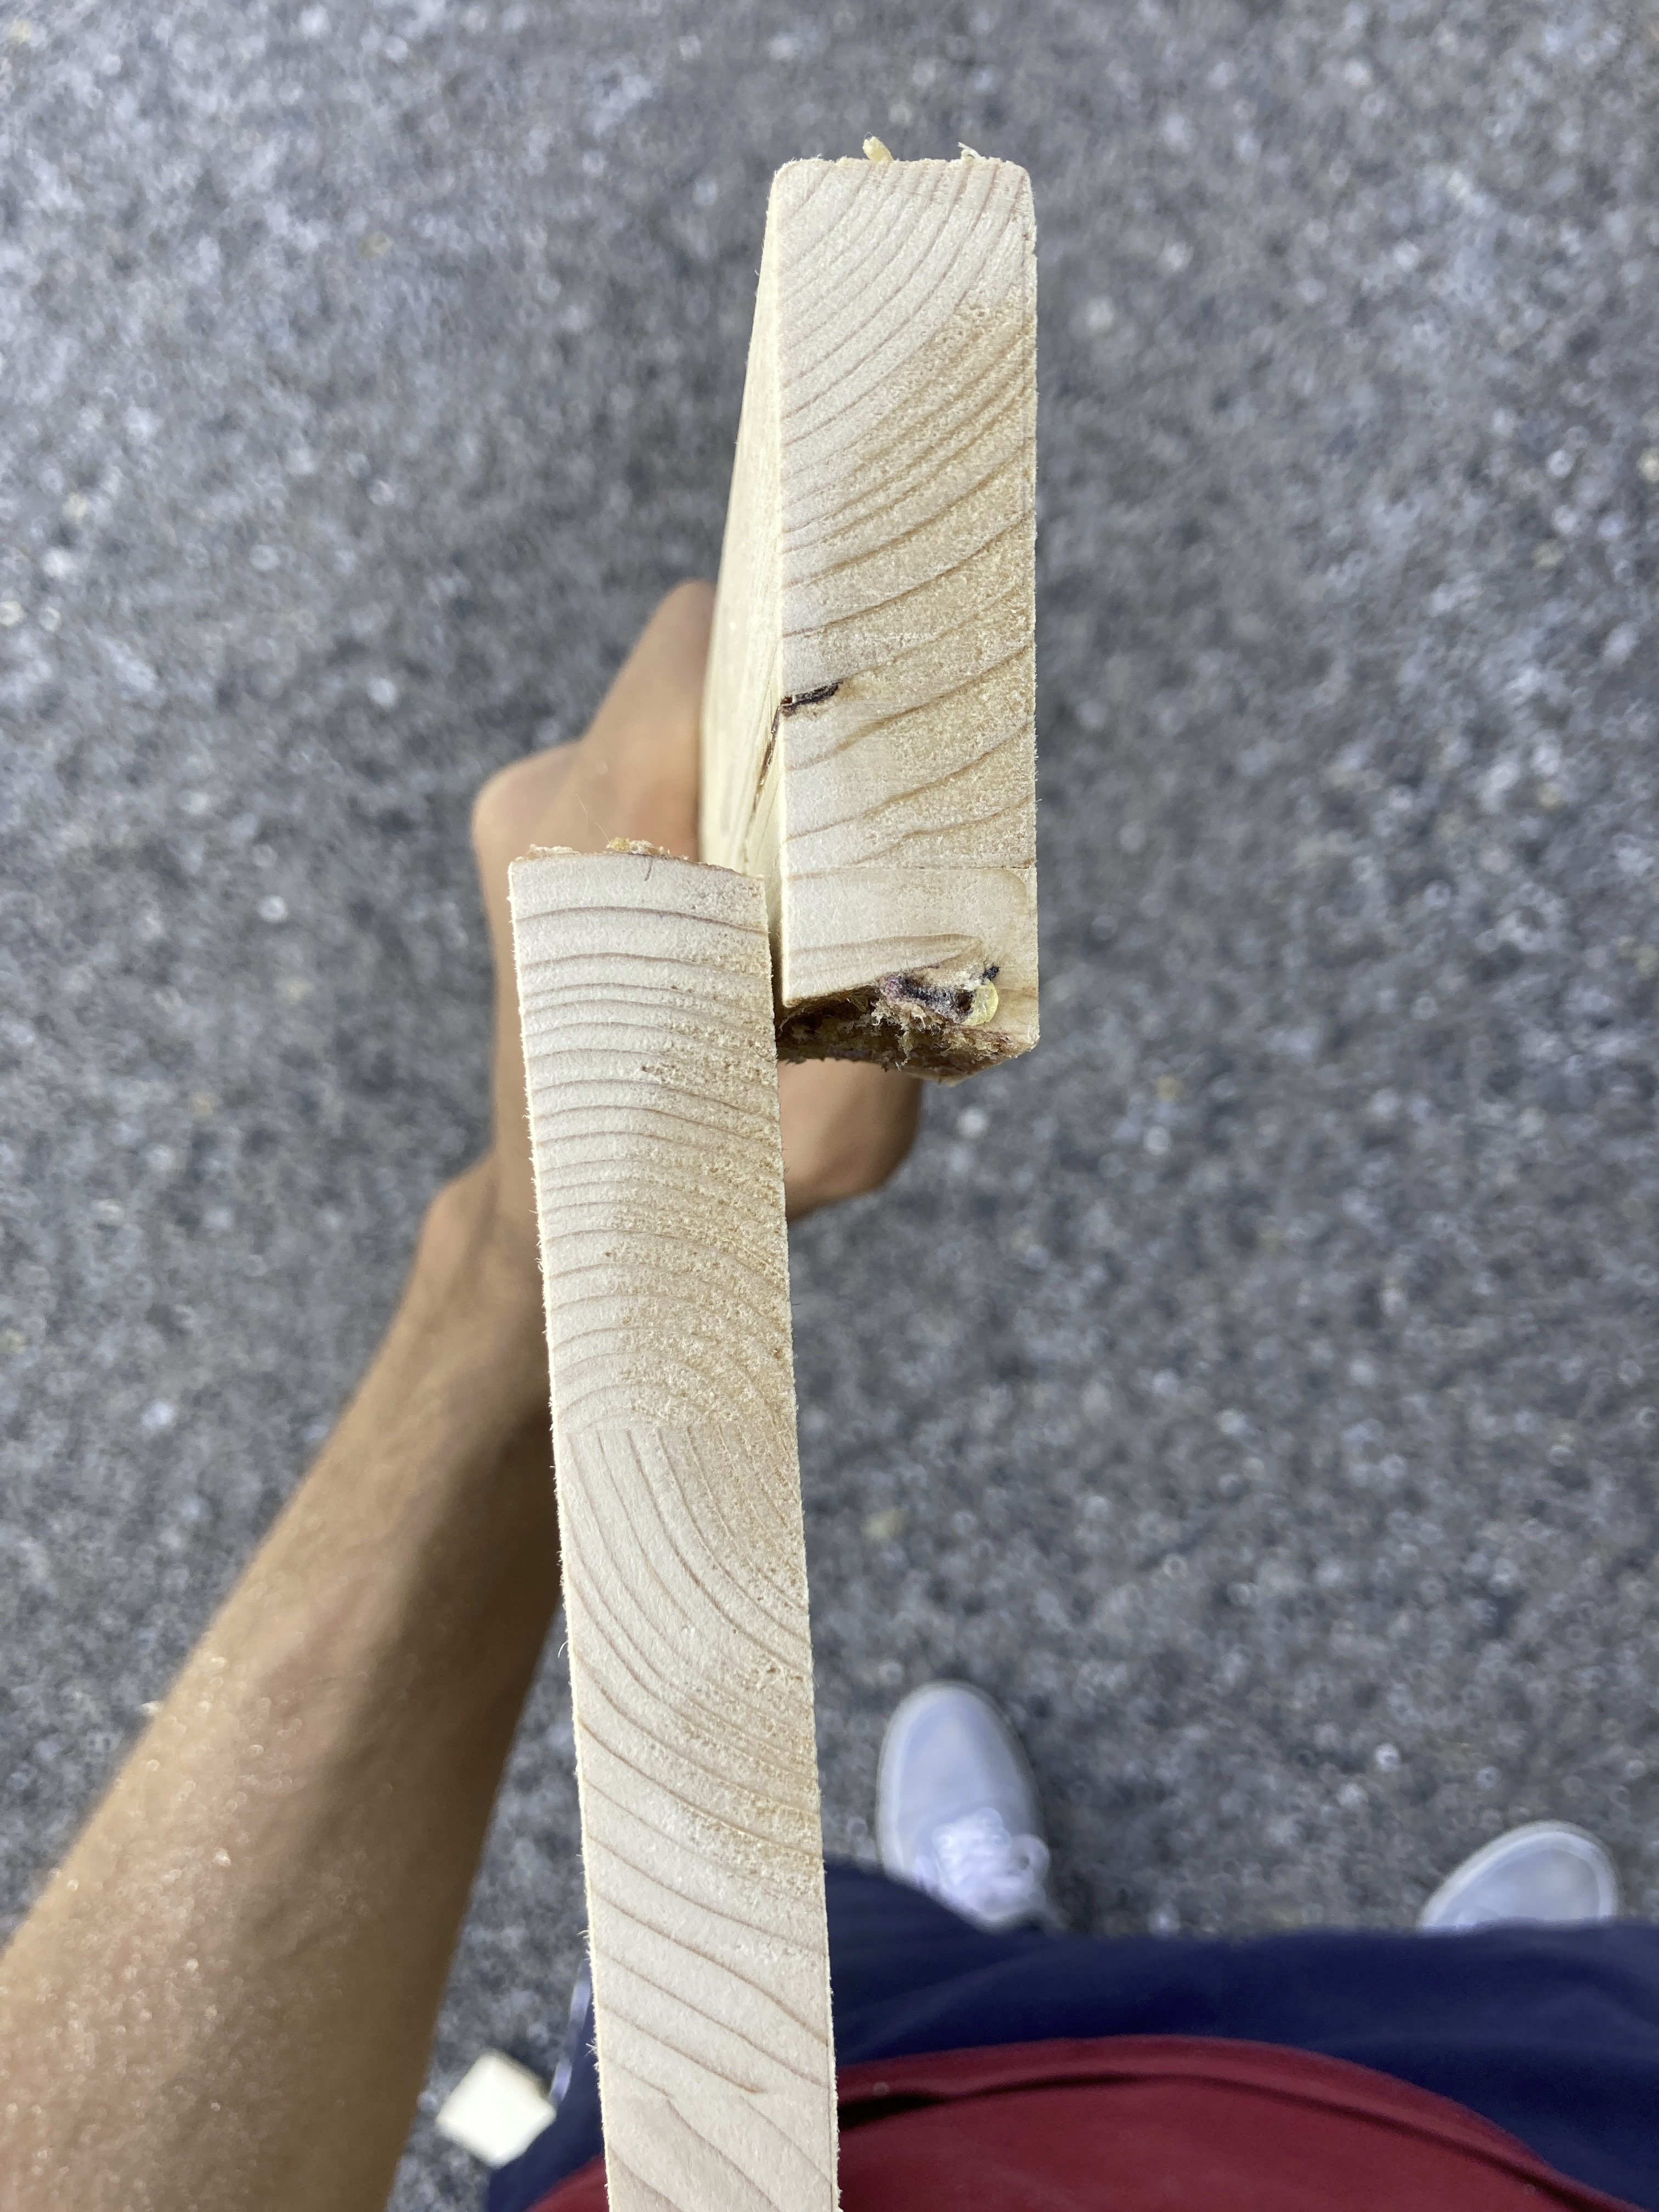
\includegraphics[width=0.25\linewidth]{bruch.png}
    \caption{Bruch eines Elements}
    \label{fig:bruch}
\end{figure}

Im Anschluss wird eine Schicht Balsaholz über die Rippen gelegt. Die verwendeten Balsaholzbrettchen haben eine Stärke von 1 mm und sind 100 cm lang. Zur Befestigung an den Spanten wird eine Tackerpistole verwendet. Durch Verspannungen im Holz ergeben sich unglücklicherweise kleinere Verformungen, welche sich negativ auf die endgültige Bootsform auswirken können.

\subsection{Glasfaserbeschichtung}
Um eine robuste Aussenhülle für das Boot zu schaffen, wird eine glasfaserverstärkte Epoxidharzschicht aufgetragen. Die Verbindung von Glasfasermatten mit Epoxidharz ergibt eine äusserst harte und stabile Schicht.  Dafür  werden die Glasfasermatten auf die Balsaholzplanken gelegt und mit Epoxidharz bestrichen. Dies führt dazu, dass die Epoxidschicht die Form des Bootes annimmt. Das unterliegende Balsaholz bildet also die formgebende und die Glasfaser-Epoxidschicht die strukturgebende Komponente. 

Dieses Vorgehen führt jedoch auch zu Problemen, da der Auftrag der Glasfaser-Epoxidschicht zu Verspannungen in der Balsaholzschicht führt. Auch die Schwankungen der Feuchtigkeit in der Werkstatt bewirken Verspannungen, welche sich dann ebenfalls auf die Balsaholzschicht auswirken.  Um diese Dellen in der Aussenhülle auszugleichen, muss sehr viel Expoxidspachtelmasse aufgetragen wird. Dafür wird eine Mischung von Expoixid und entsprechendem Härtungsmittel verwendet.  Um das folgende Plan schleifen der Oberfläche zu vereinfachen, werden diesem Gemisch Microballons beigemischt und ein Tixotropiermittel wird zugegeben, um das Gemisch einzudicken. Der Prozess des Auftragens und Abschleifens muss viele Male wiederholt werden. Das ist sehr zeitaufwändig, da immer gewartet werden muss, bis die neu aufgeragenene Schicht vollständig getrocknet ist.  Dabei wird versucht einen möglichst glatten, stromlinienförmigen Körper zu formen.

Um eine Asymmetrie beim Bug zu vermeiden, wird sehr viel \\Expoxid-Spachtelmasse aufgetragen. Kleine Glasfaserschnippsel, welche zur Spachtelmasse dazugerührt werden, geben dieser weitere Stabilität, damit der Bug gut geschützt ist.

Zum Schluss wird der Bootskörper mit Sperrholzplatten abgedeckt. Diese werden in einem ersten Schritt auf den offenen Bootskörper gelegt. Dann werden mit einem Bleistift die Konturen des Bootskörpers nachgezogen. Die Deckplatten werden entlang der Bleistiftmarkierungen ausgesägt. In der Mitte des Boots wird eine Öffnung in die Deckplatten gesägt und die Deckplatten mit dem Schiffskörper verleimt. Die vorhandene Lücke im Deck wird erst nach dem Einbau des Masts und der Elektronik und der Bemalung der Deckplatte mit einer weiteren abnehmbaren Sperrholzplatte verschlossen. Am Schluss werden noch die Positionslampen angebracht. 
\subsection{Ruder}
Das Ruder wird aus einer Tannen-Leimholz-Platte ausgesägt. Dabei wird daselbe Verfahren wie bei den Spanten angewendet. Anschliessend wird das Werkstück mit der Schleifmaschine bearbeitet und in Form gebracht. 
\begin{figure}[H]
    \centering
    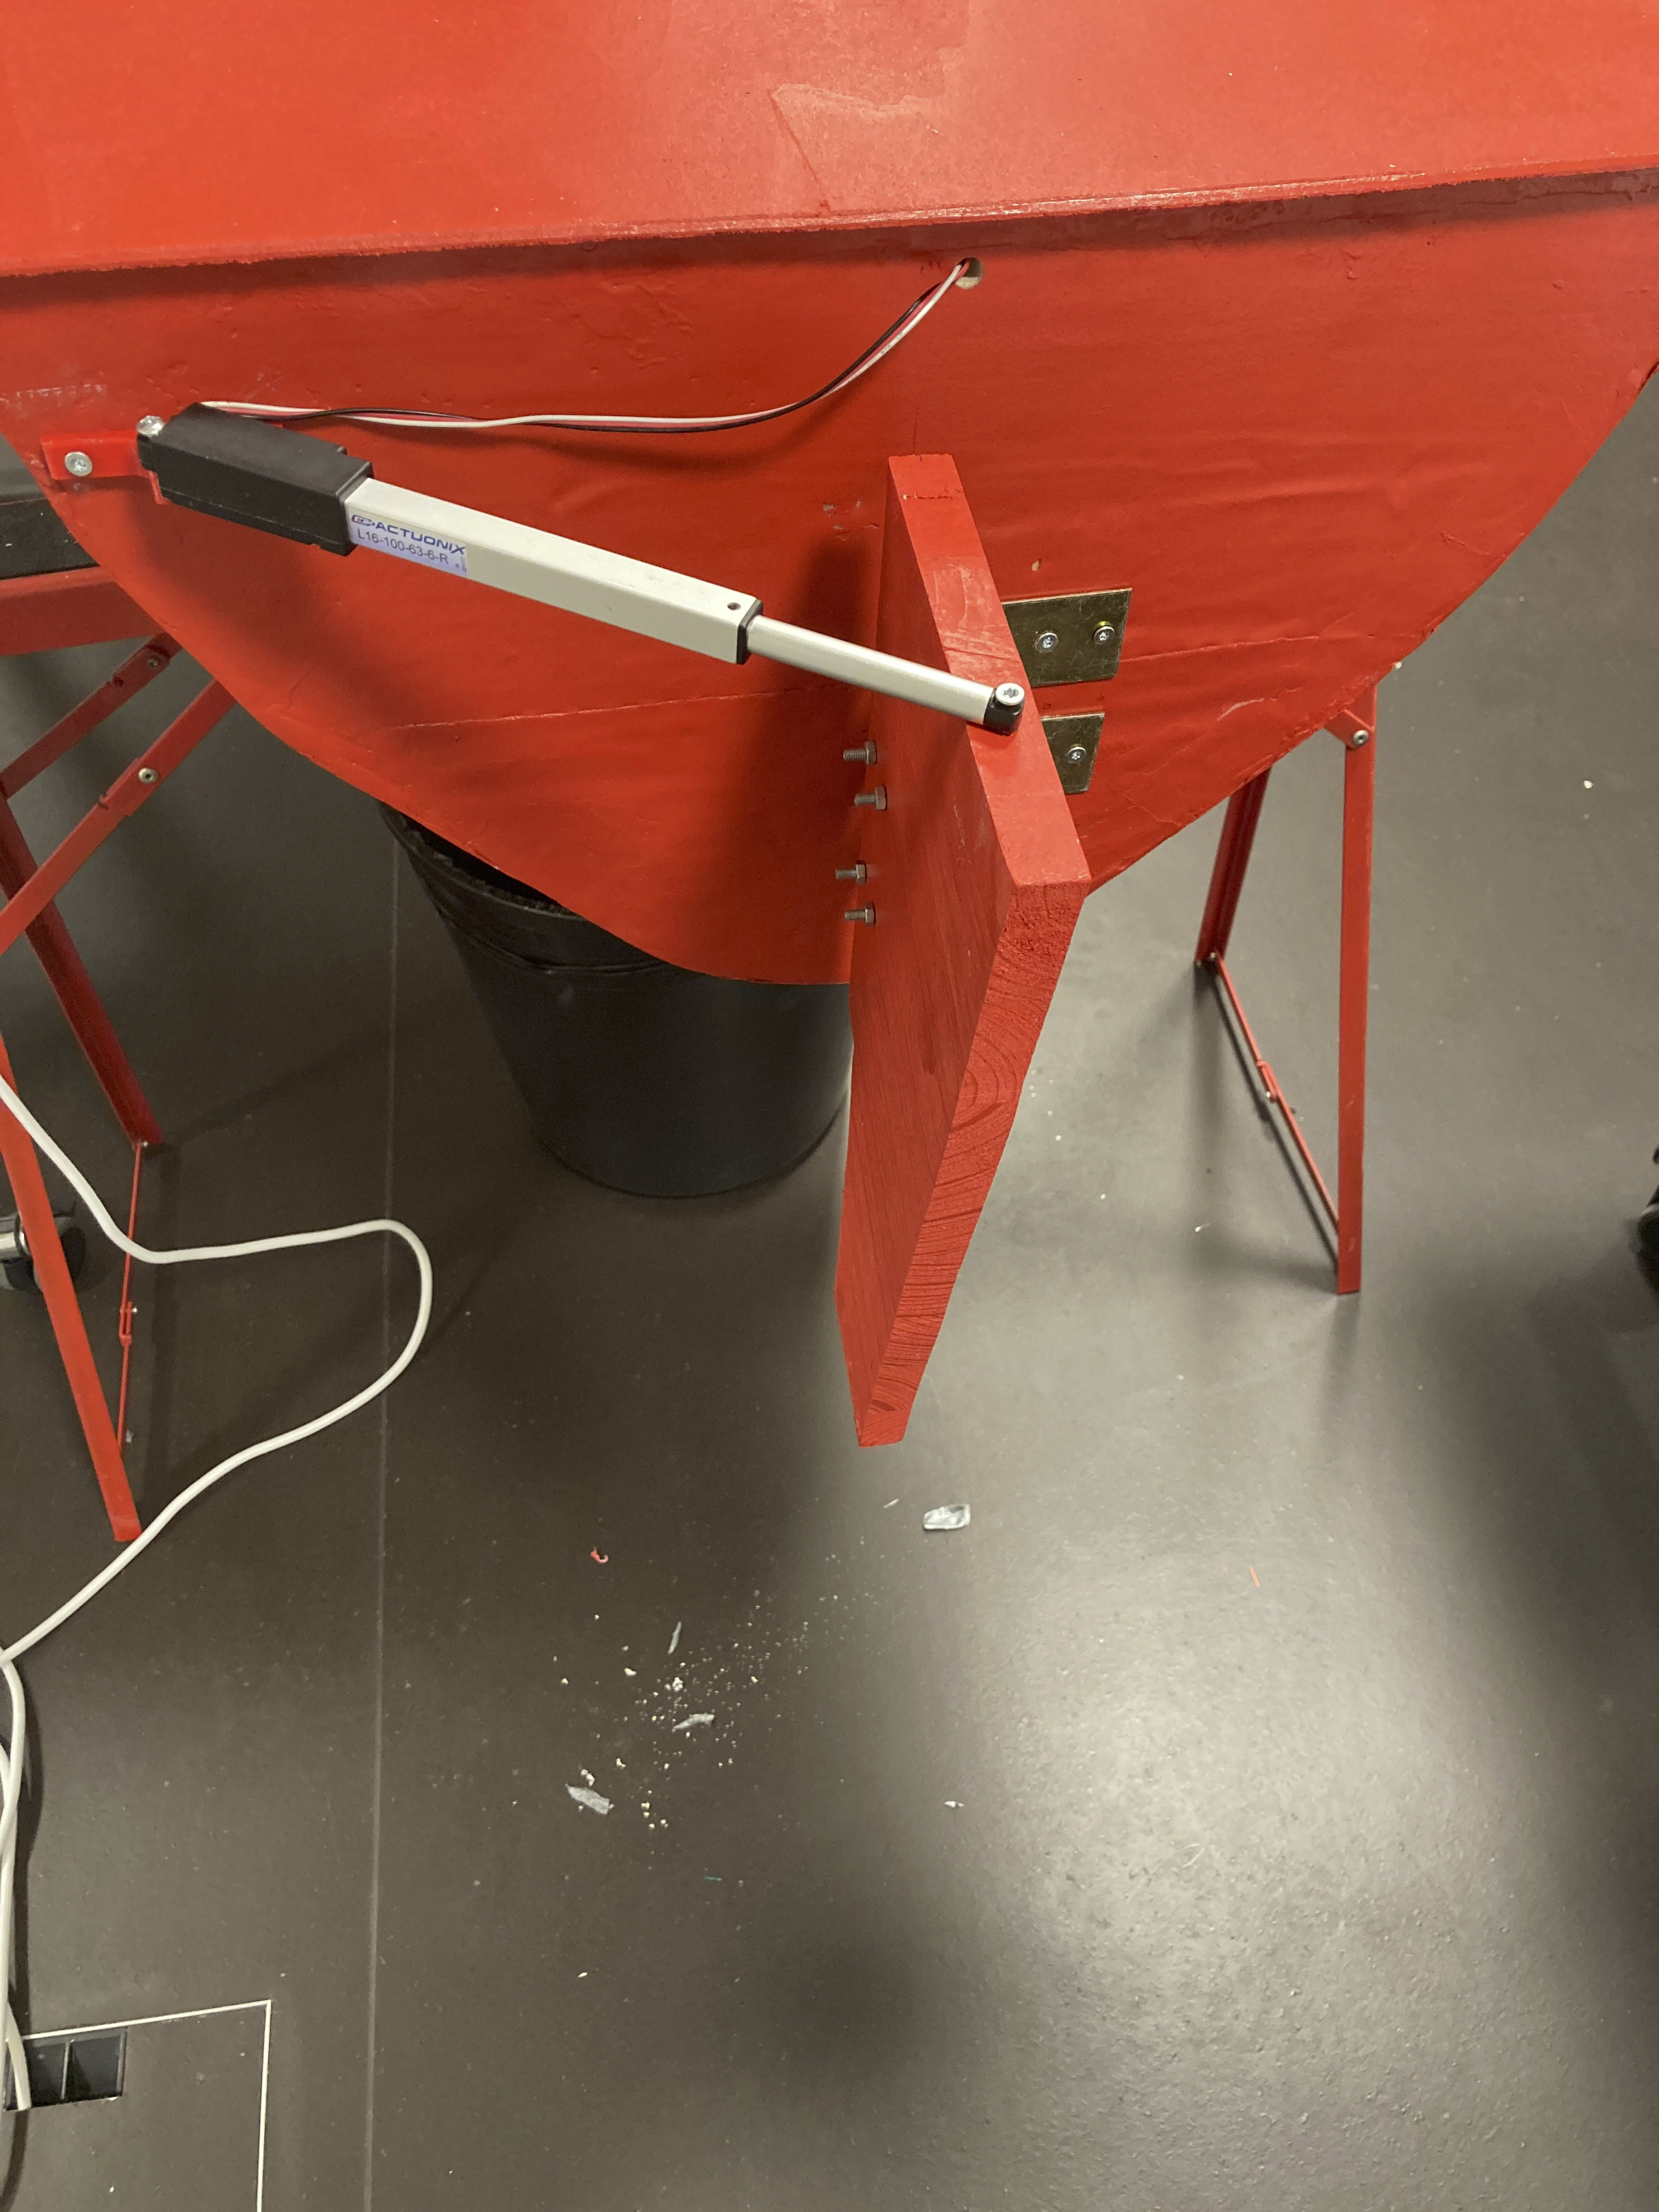
\includegraphics[width=0.5\linewidth]{assets/ruderimagegrafik.png}
    \caption{Fertiger Einbau des Ruders}
    
\end{figure}

Nach der Lackierung mit roter Farbe wird das Ruder am Heck des Schiffskörpers befestigt und mit der Welle des Aktuators verbunden.
\subsection{Kiel}
%In einem ersten Schritt werden die 5 Bretter ausgesägt, miteinander verleimt und verschraubt. Anschliessend werden in die Löcher für die Gewindestangen in die beiden äusseren Kielbretter gebohrt. 

%Im nächsten Schritt wird ein Loch in jedes der beiden 2 kg Gewichte gebohrt. So können die Gewichte mit dem Kielhauptbrett verschraubt werden. Nach dem Druck der beiden Schutzgehäuse werden diese über die Gewichte gestülpt und mit dem Kielhauptbrett verleimt.    
%\begin{figure} [H]
%    \centering
%    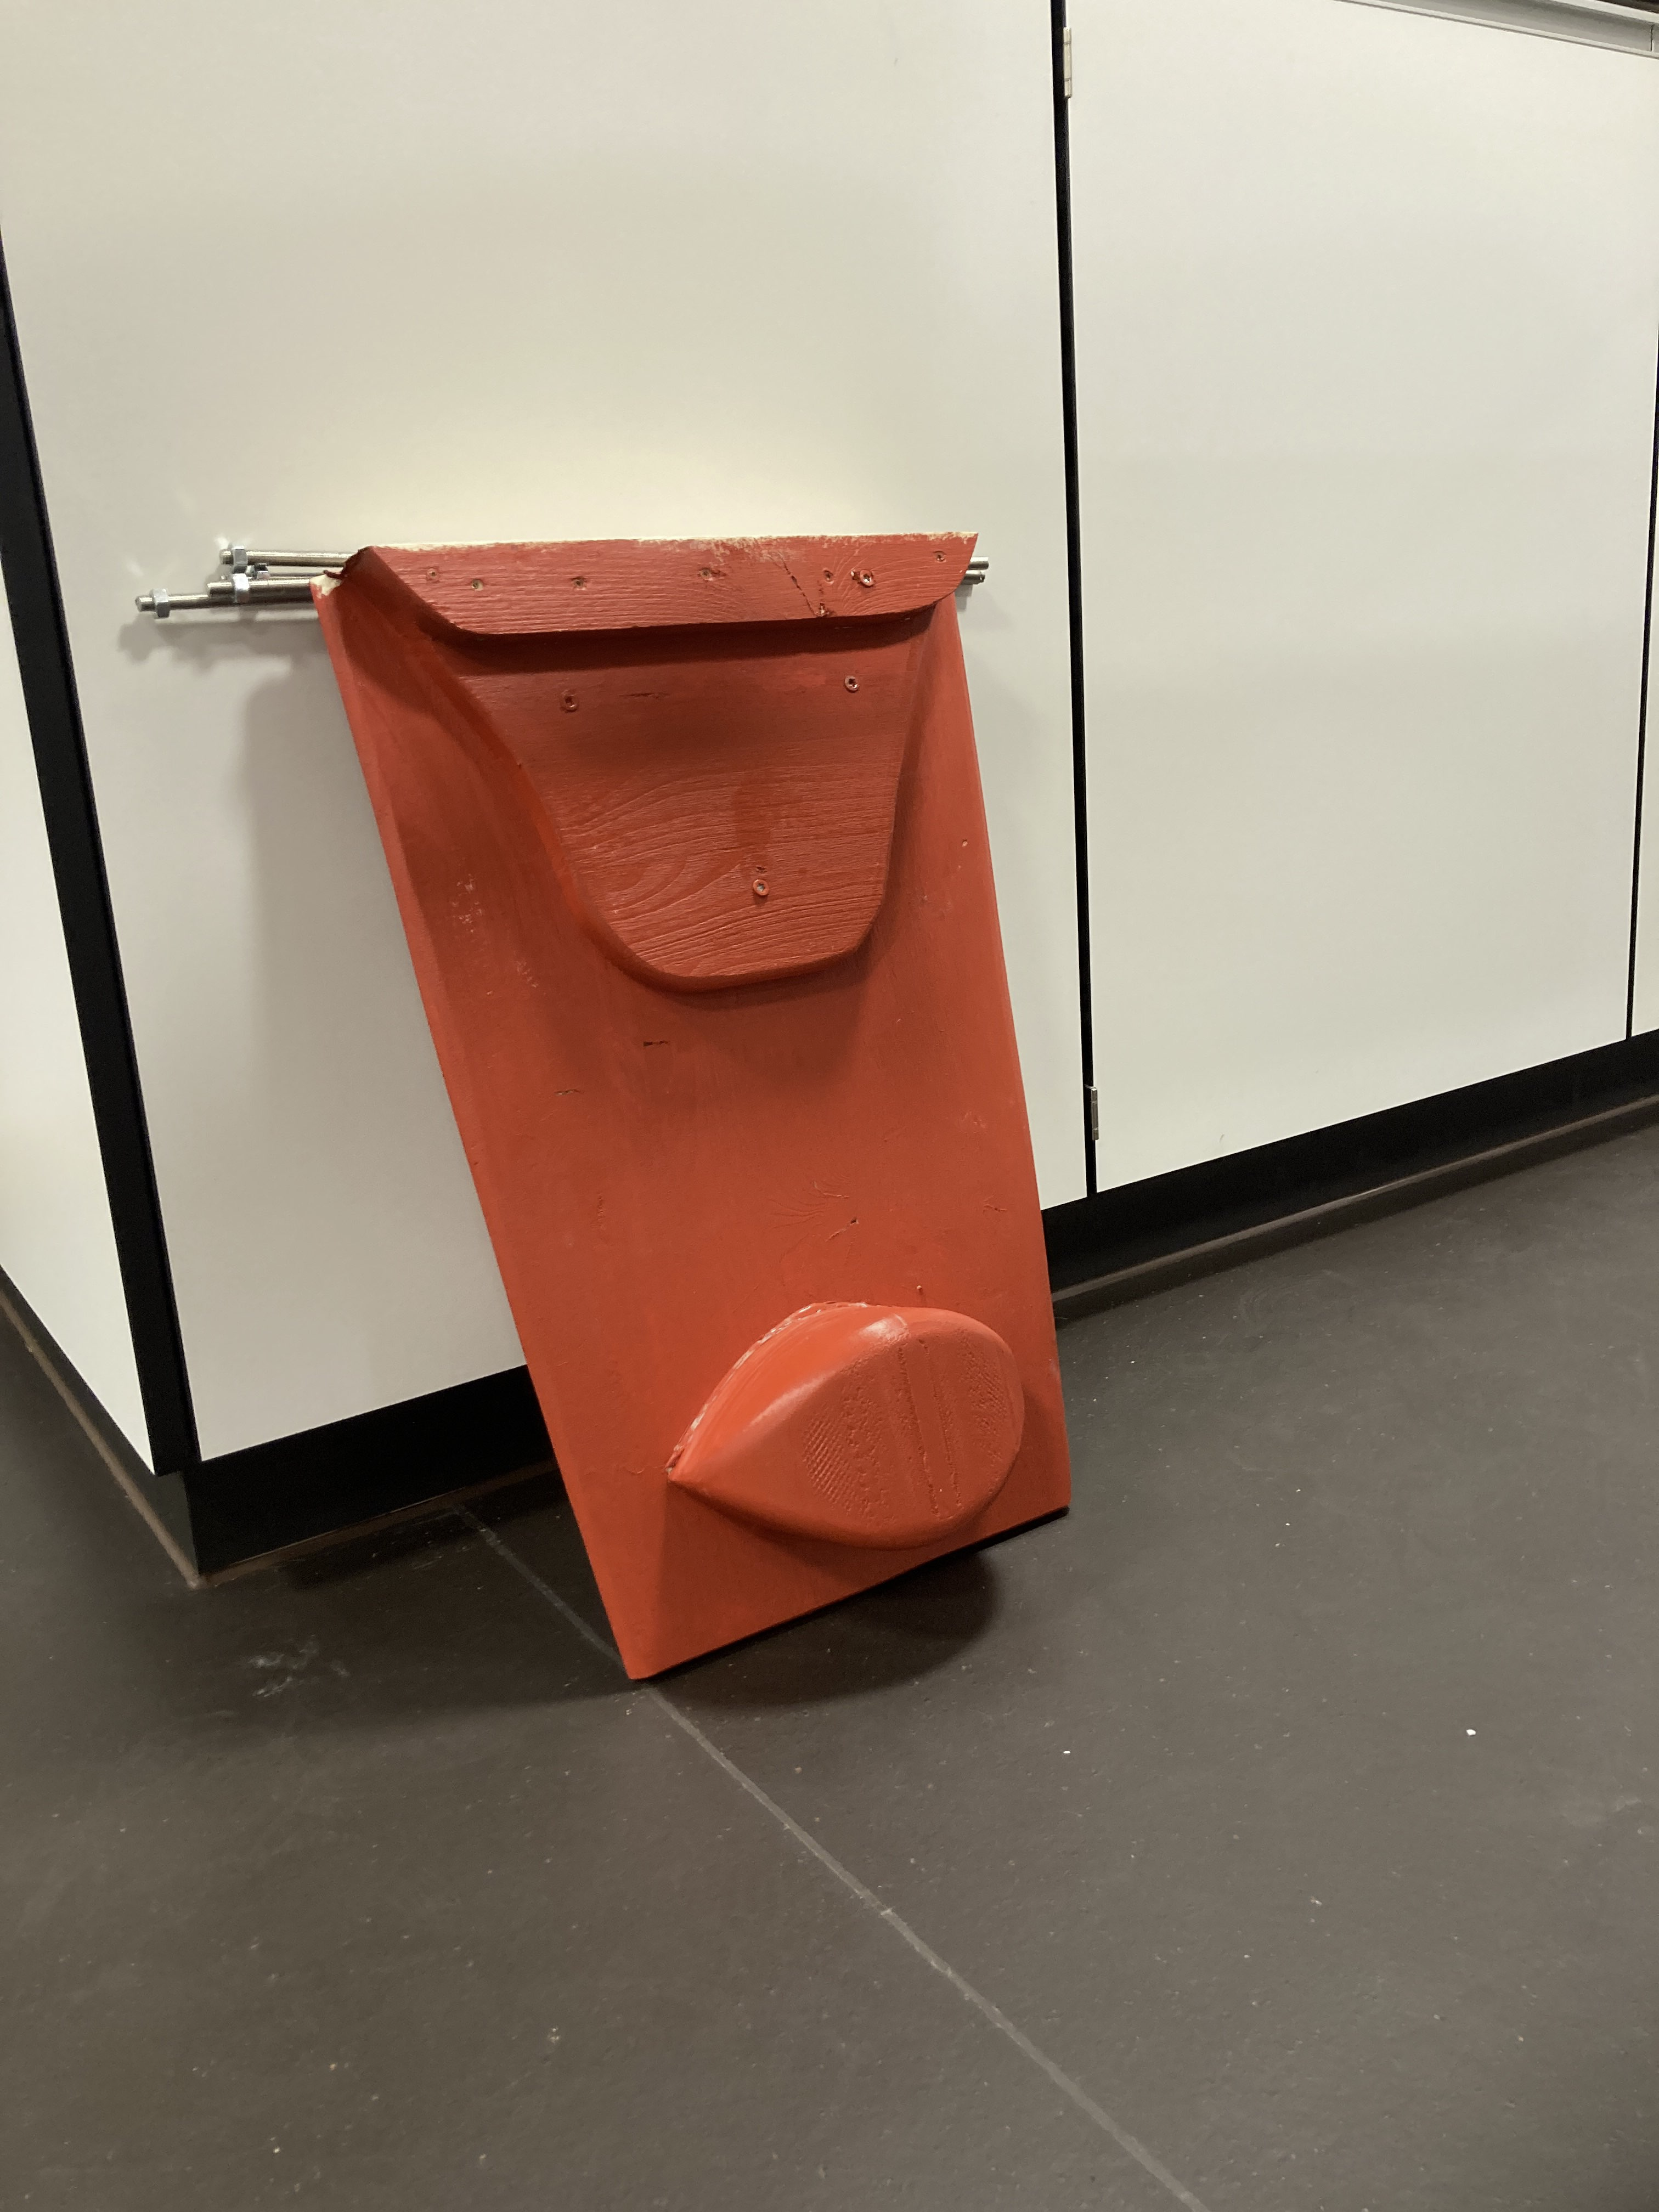
\includegraphics[width=0.3\linewidth]{assets/Kiel_lakiert.png}
%    \caption{Fertiger Kiel}
%    \label{fig:enter-label}
%\end{figure}
Damit der Kiel die nötige Stabilität bereitstellen kann, wird ein Balastkiel verwendet. Balastkiele bestehen aus einem Gewicht welches möglichst tief unter dem Schiff liegt. Dafür wurde eine Stützstruktur aus Edelstahl gebaut. Es werden zwei Stahlstangen mit schäg-positionierten kürzeren Profilen verschweisst. Somit wird eine Fachwerkstruktur erzeugt.
Der gewählte Stahl entspricht der DIN 1.4016 Norm. Dieser ist bekannt für seine relativ hohe Korrosionsbeständigkeit.\cite{MAR2025STEEL}

Damit der Kiel das nötige Gewicht hat, wird aus Blech eine Hohlform geformt. Diese ist von einem Eisenplastiker geformt worden. Anschliessend wird diese mit Weichblei gefüllt. 

Damit der Kiel im Wasser nicht zu viel Wiederstand erzeugt, werden 3D gedruckten, symmetrischen Wände angebracht. Um Wassereintritt in den Kiel zu vermeinden, wird dieser mit einem wasserfesten Bauschaum aus dem Baumatkt gefüllt. Dies verhindert zusätzlich, dass mögliche Korrosion im innernen des Kiels, die strukturelle Stabilität gefährdet.
Da 3D gedruckte Teile nicht die nötige Stabilität liefern, wird zusätzlich eine doppelte Glasfaserverstärkung verbaut. 

Der Kiel wird über vier M12 Schrauben mit dem inneren des Bootskörpers verbunden. Im inneres des Bootes werden zwei Flachstahlprofile verbaut an welchen dem Kiel festgeschraubt wird. 

%% TODO Bilder




\section{Segel}

\section{Hauptsegel}
Das Segel besteht grundsätzlich aus 4 zusammengeklemten EPS platten. EPS wurde gewählt, da dieser deutlich weniger porös ist als XPS. In einem vorherigen Versuch zum Bau des Segels wurden XPS platten verwendet und von Hand ausgeschnitten. Die Ungenauigkeit, die das Schneiden von Hand verursacht hat und Porösität haben zu keinem zufriedenstellendem Ergebnis geführt.
\\
In der neuen Iteration sind nun jeweils zwei Platten zusammengeklebt. Da die EPS Form aber vorallem Form und nicht strukturtragend ist, wird eine Schicht Glasfasermatten laminiert. Das Segel verfügt somit über genügend Stabilität und resistenter gegen die Witterung.
Es wird eine sehr feinmaschiges Glasfaserlaminat verwendet, da dies eine glattere Oberflächenstruktur ermöglicht.Da jedoch kein Werkzeug zur Vakumierung verfügbar war, konnte das entstehen einiger Luftblasen nicht vermieden werden. 


\section{Falp}
Das Flap ist ebenfalls mit einer CNC Maschine aus EPS Kunstschaum gefräst. Da aufgrund der Konstruktionsweise kein Mast gebraucht wird, kann grundlegend auf zwei zusammengeklebten Platten verzichtet werden.
Das Flap ist aus einer einzigen Platte, welche beidseitig gefräst ist.
Im Anschluss wird auch das Flap mit einer Schicht Glasfasermatten überdeckt.




\section{Bemalung}
Da das autonome Segelboot gut sichtbar sein soll, wird es in roter Signalfarbe bemalt. Dazu wird seidenmatter Acryllack verwendet, der mithilfe einer Farbwalze auf den Bootskörper aufgetragen wird. Es wurde bewusst eine matte Farbe gewählt, da diese kleine Ungenauigkeiten und Dellen in der Bootsform besser kaschiert als glänzende Farben. 

Da das Ruder der Kiel und das Deck keine Schutzhülle aus glasfaserverstärktem Epoxidharz verfügen, hat die Farblackierung bei diesen Bauteilen auch eine Schutzfunktion.

Erst wenn die Farbe trocken ist, wird am Bug der Schiffsname Panta Exo aufgemalt. Dazu wird eine Schablone erstellt und verwendet. 
\section{Einbau der Elektronik}
Als erstes wird ein digitaler Schaltplan mit allen Sensoren und Aktuatoren und Sensoren erstellt. Dieser dient ursprünglich für den Bau der Platine, kann für den Einbau der Ekeltronik jedoch wiederverwendet werden.
\subsection{Platine}
Die Platine wird in eine Kunststoffbox verbaut und in den Bootskörper gesetzt. Alle Sensoren werden über die Steckverbindungen verbunden.
\subsection{GPS}
Das GPS Modul wird in eine eigene Kunststoffbox auf dem Deck verbaut. Als das GPS in der nähe der am Gehäuse festgemacht BLE Antenne war, war der Empfang des GPS limitiert. Es kann keine direkte Korrelation festgestellt werden, jedoch wurden keine Probleme seit der Änderung Festgestellt, weshalb dies so belassen wird.  
\subsection{Aktuatoren}
Der Aktuator für das Ruder wird am Heck des Bootes am Achtersteven befestigt. Seine Welle wird mit dem Ruder verbunden. Das Ruder kann bis zu einem Winkel von etwa 60 Grad eingeschlagen werden.
Der Einbau des zweiten Aktuators wird oben beim Bau des Sailflap beschrieben. Seine Steuerkabel werden durch das Gosssegel in den Mast und von dort durch den Schleifring in den Bootskörper geführt.
\subsection{Energieversorgung}
Der Akku wird in die gleiche Kurstoffbox wie die Platine verbaut. Box verfügt über einen doppelten Boden.


\begin{figure}
    \centering
    \includegraphics[width=0.5\linewidth]{assets/electronics housing.png}
    \caption{Elektronik Gehäuse}
    \label{fig:enter-label}
\end{figure}